\section{Uniform Stability Calculus}
\label{sec:uniform-calculus}

At the level of perturbation operations, replace-one is the composite move
obtained by deleting an occurrence and then inserting a new labeled point.
That observation is almost tautological at the sample level, but it is worth
writing down explicitly because it yields the correct direction of implication
for worst-case stability control.

\begin{figure}[t]
    \centering
    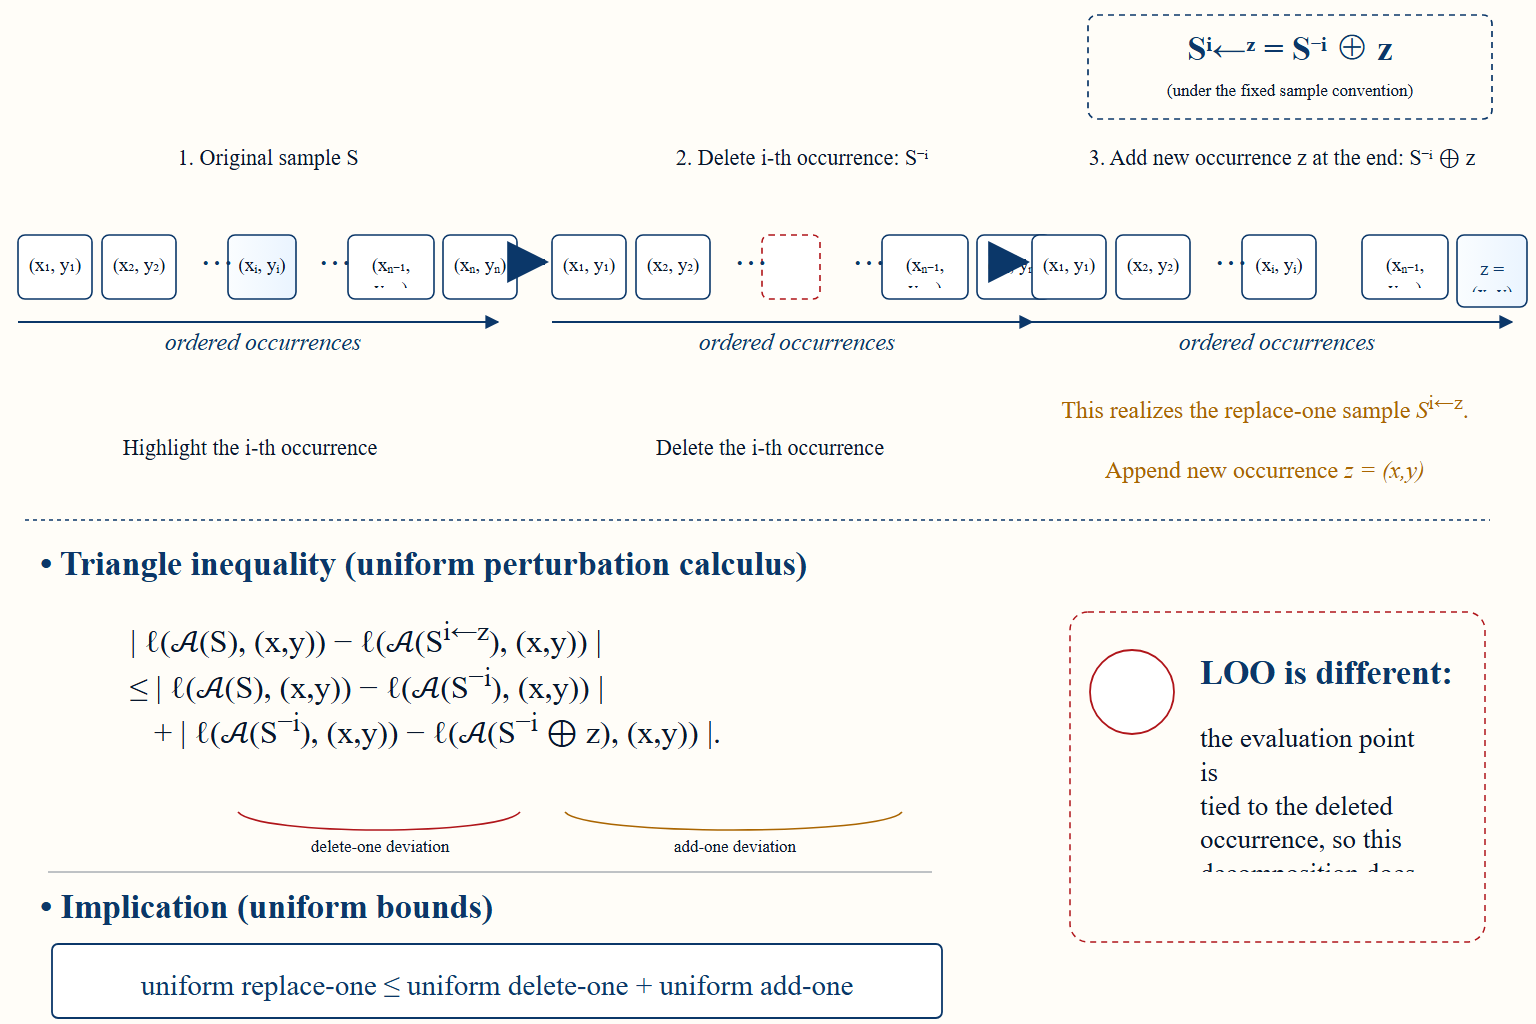
\includegraphics[width=0.78\linewidth]{outputs/figures/recreated_fig03.png}
    \caption{Operation-level factorization of a replace-one perturbation into a
    delete-one step followed by an insert-one step. The proof of
    \cref{prop:4.1} is just the triangle inequality on the
    corresponding binary losses.}
    \label{fig:uniform-calculus}
\end{figure}

\begin{note}[Insert-One Operation]
For an ordered tuple $T$ of size $m$ and any labeled point $z \in X \times \{0,1\}$, the result of inserting $z$ at position $j \in \{1,\ldots,m+1\}$ is denoted $T \oplus_j z$. The notation $S^{i\leftarrow z} = (S^{-i}) \oplus_i z$ means: first delete occurrence $i$ from $S$, obtaining $S^{-i}$, then insert $z$ at the original position $i$ of the deleted occurrence. This preserves the ordered structure and aligns with the in-place replacement semantics.
\end{note}

\begin{note}[Uniform insert-one stability]
When we speak of bounded insert-one stability $\beta_{\ins}(n)$ uniformly over all insertion positions, we mean: for every ordered sample $T$ of size $m$, every insertion position $j \in \{1,\ldots,m+1\}$, every labeled point $z$, and every query-label pair $(x,y)$,
\[
\left|\ell(A(T),(x,y)) - \ell(A(T \oplus_j z),(x,y))\right| \le \beta_{\ins}(m).
\]
The bound may depend on the sample size $m$ before insertion.
\end{note}

\begin{proposition}[Uniform replace-one via delete-and-insert]
\label{prop:4.1}
Fix a deterministic learning rule $A$ that maps ordered samples to predictors
and a bounded loss $\loss \in [0,1]$. Suppose that:
\begin{enumerate}[leftmargin=*,label=(\arabic*)]
    \item Delete-one stability is bounded by $\beta_{\del}(n)$ uniformly over all ordered samples of size $n$, all indices, and all query-label pairs.
    \item Insert-one stability is bounded by $\beta_{\ins}(n)$ uniformly over all ordered samples of size $n$, all insertion positions $j$, all admissible labeled points $z$, and all query-label pairs.
\end{enumerate}
Then every replace-one perturbation satisfies
\[
\left|\loss(A(S),(x,y))-\loss(A(S^{i\leftarrow z}),(x,y))\right|
\le \beta_{\del}(n)+\beta_{\ins}(n-1).
\]
\end{proposition}

\begin{note}[Proof sketch for \cref{prop:4.1}]
For fixed $S,i,z,(x,y)$, let $T=S^{-i}$. By the insertion convention,
$S^{i\leftarrow z}=(S^{-i})\oplus_i z$. Therefore
\begin{align*}
\left|\loss(A(S),(x,y))-\loss(A(S^{i\leftarrow z}),(x,y))\right|
&\le
\left|\loss(A(S),(x,y))-\loss(A(T),(x,y))\right| \\
&\quad +
\left|\loss(A(T),(x,y))-\loss(A(T\oplus_i z),(x,y))\right| \\
&\le \beta_{\del}(n) + \beta_{\ins}(n-1)
\end{align*}
by the triangle inequality and the uniform assumptions. The last line uses
that $S^{-i}$ has size $n-1$, so the insert-one bound applies with that sample
size.
\end{note}

\Cref{prop:4.1} is deliberately abstract. It is not specific to
$k$-NN, and it does not by itself tell us whether the bound is informative for a
particular local learner. Its role is to record the algebra of perturbation
types before we examine the combinatorics of deterministic nearest
neighbors.

The proposition also clarifies what it does \emph{not} say. A pointwise LOO
indicator cannot simply be dropped into the role of delete-one control above,
because LOO changes the evaluation point along with the sample. Similarly, a
fresh-test or expected-loss stability statement from the classical literature
does not automatically transfer to the worst-case fixed-query indicators used
in the present paper. The whole point of the calculus is to prevent these
invalid transfers between notions.
